\chapter{Signal and background modelling}
\label{chap:sigbkg}

\section{Introduction}

The final results of this analysis are extracted by performing a maximum likelihood fit 
of the signal and background models to the diphoton invariant mass distribution observed in data.
In this fit, the value of twice the negative log-likelihood (2NLL) is minimised 
for each value of the parameter to be measured.
The resulting 2NLL curve can be used to extract the best-fit value and uncertainty 
of the parameter of interest.
In addition, systematic uncertainties are included in the fit to account for 
imperfect knowledge of both theoretical and experimental inputs to the analysis.
These uncertainties are implemented in the form of nuisance parameters.
A nuisance parameter is a variable which affects the measured value 
but is not in itself of any interest.
In the final fit, nuisance parameters are ``profiled".
This means their values are allowed to vary, 
either freely or with an additional constraint applied 
which penalises deviation from the nominal expectation.
This has the effect of widening the 2NLL curve and thereby increasing the overall uncertainty
on a given measurement.
Full details of the the statistical procedure used to extract the results 
are given in Chapter~\ref{chap:results}.

In order to perform the fits, models of the signal and background \mgg distributions 
in each analysis category are required as inputs.
The signal model is derived from simulation, 
with a model constructed for each particle level stage 1 cross section bin 
in each reconstructed analysis category.
Both the shape and normalisation of the model are parameterised as a function of \mH.
The data-driven background model considers a range of different functional forms to 
represent the smoothly falling background spectrum, 
following the approach described in Ref.~\cite{Envelope}.
This methodology follows that used in the previous CMS \Hgg analysis, 
which is described in Ref.~\cite{HIG-16-040}.
The construction of both the signal and background models is described in detail in this chapter.
In addition, the treatment of systematic uncertainties affecting the two models is discussed.

\section{Signal modelling}

The signal model is a parametric function of \mH which describes the shape of the \mgg distribution, 
together with the expected normalisation of this shape.
An independent model is constructed for each stage 1 bin in each analysis category
Additionally, since the \mgg shape depends on whether the right vertex (RV) 
or wrong vertex (WV) has been chosen, the model for each of these cases is constructed separately.

Each model consists of a sum of up to five Gaussian functions.
The number of Gaussian functions required depends on the shape of the \mgg spectrum 
and the available quantity of simulated events.
Alternative functional parameterisations have been studied, 
such as the sum of a Gaussian function to represent the core of the \mgg distribution 
and an exponential to model each tail \cite{LouieThesis}.
This alternative parameterisation yields very similar signal models to the sum of Gaussian functions, 
and the final results are unaffected.
The Gaussian-based model is retained due to its simplicity and computational efficiency.

The parameters of the Gaussian functions are determined by performing a fit 
to the simulated \mgg distribution for each model.
In order to account for the fact that the mass of the Higgs boson is not known exactly, 
the model constructed is a continuous parametric function of \mH.
The dependence on \mH is determined by simultaneously fitting events simulated with 
three values of \mH: 120, 125, and \SI{130}{GeV}.
Each parameter of each Gaussian function is represented as a linear function of \mH; 
the shape of each model then consists of $2\left(3N_{\textrm{Gaus}}-1\right)$ parameters, 
where $N_{\textrm{Gaus}}$ is the chosen number of Gaussian functions.
The values of these parameters are established by the simultaneous fit across mass points.
An example of the evolution of signal model shapes as a function of \mH, 
for the ggH 0J bin the 0J Tag 0 category, is shown in Figure~\ref{fig:sigbkg_interp}
By construction, the shape and normalisation of the models vary smoothly with \mH.

\begin{figure}[hptb]
  \centering
  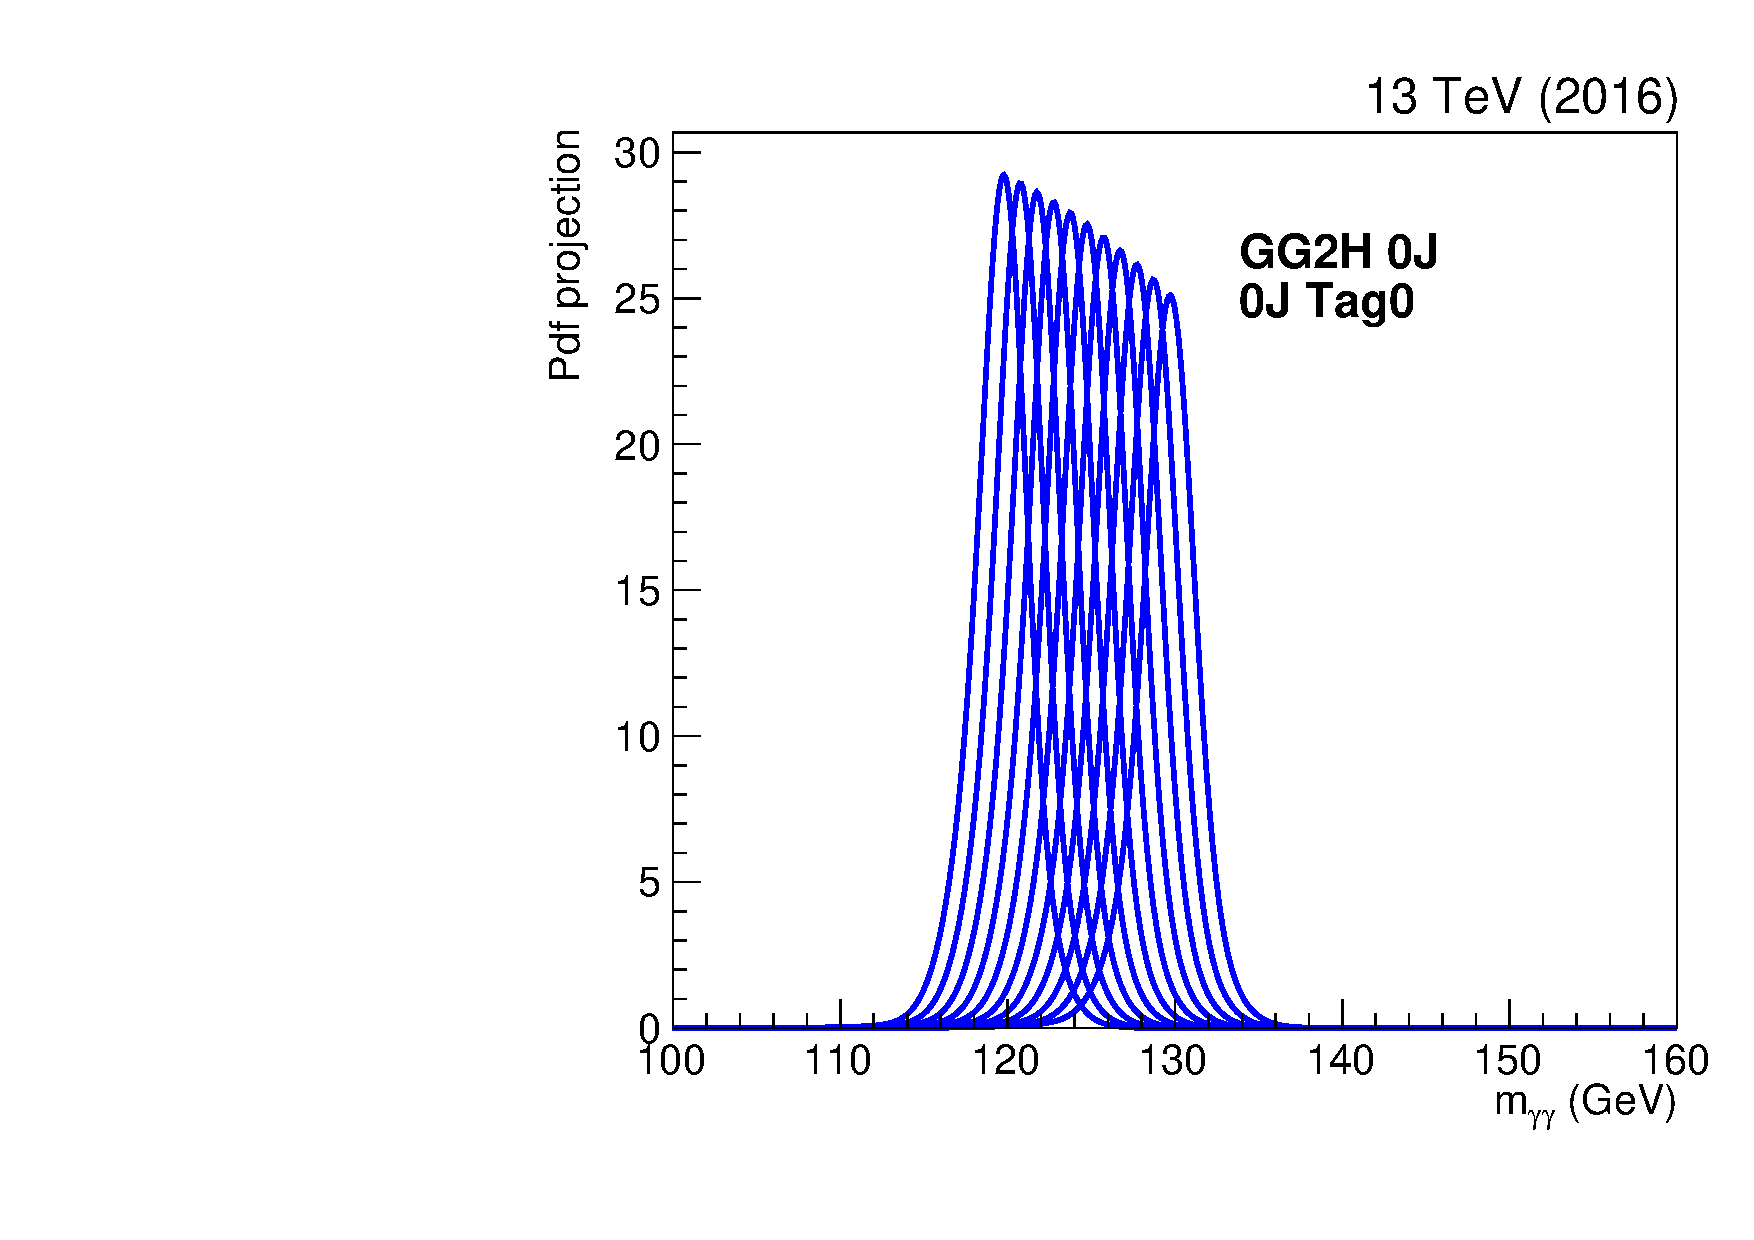
\includegraphics[width=0.49\textwidth]{Figures/SigBkg/GG2H_0J_RECO_0J_Tag0_interp_2016.pdf}
  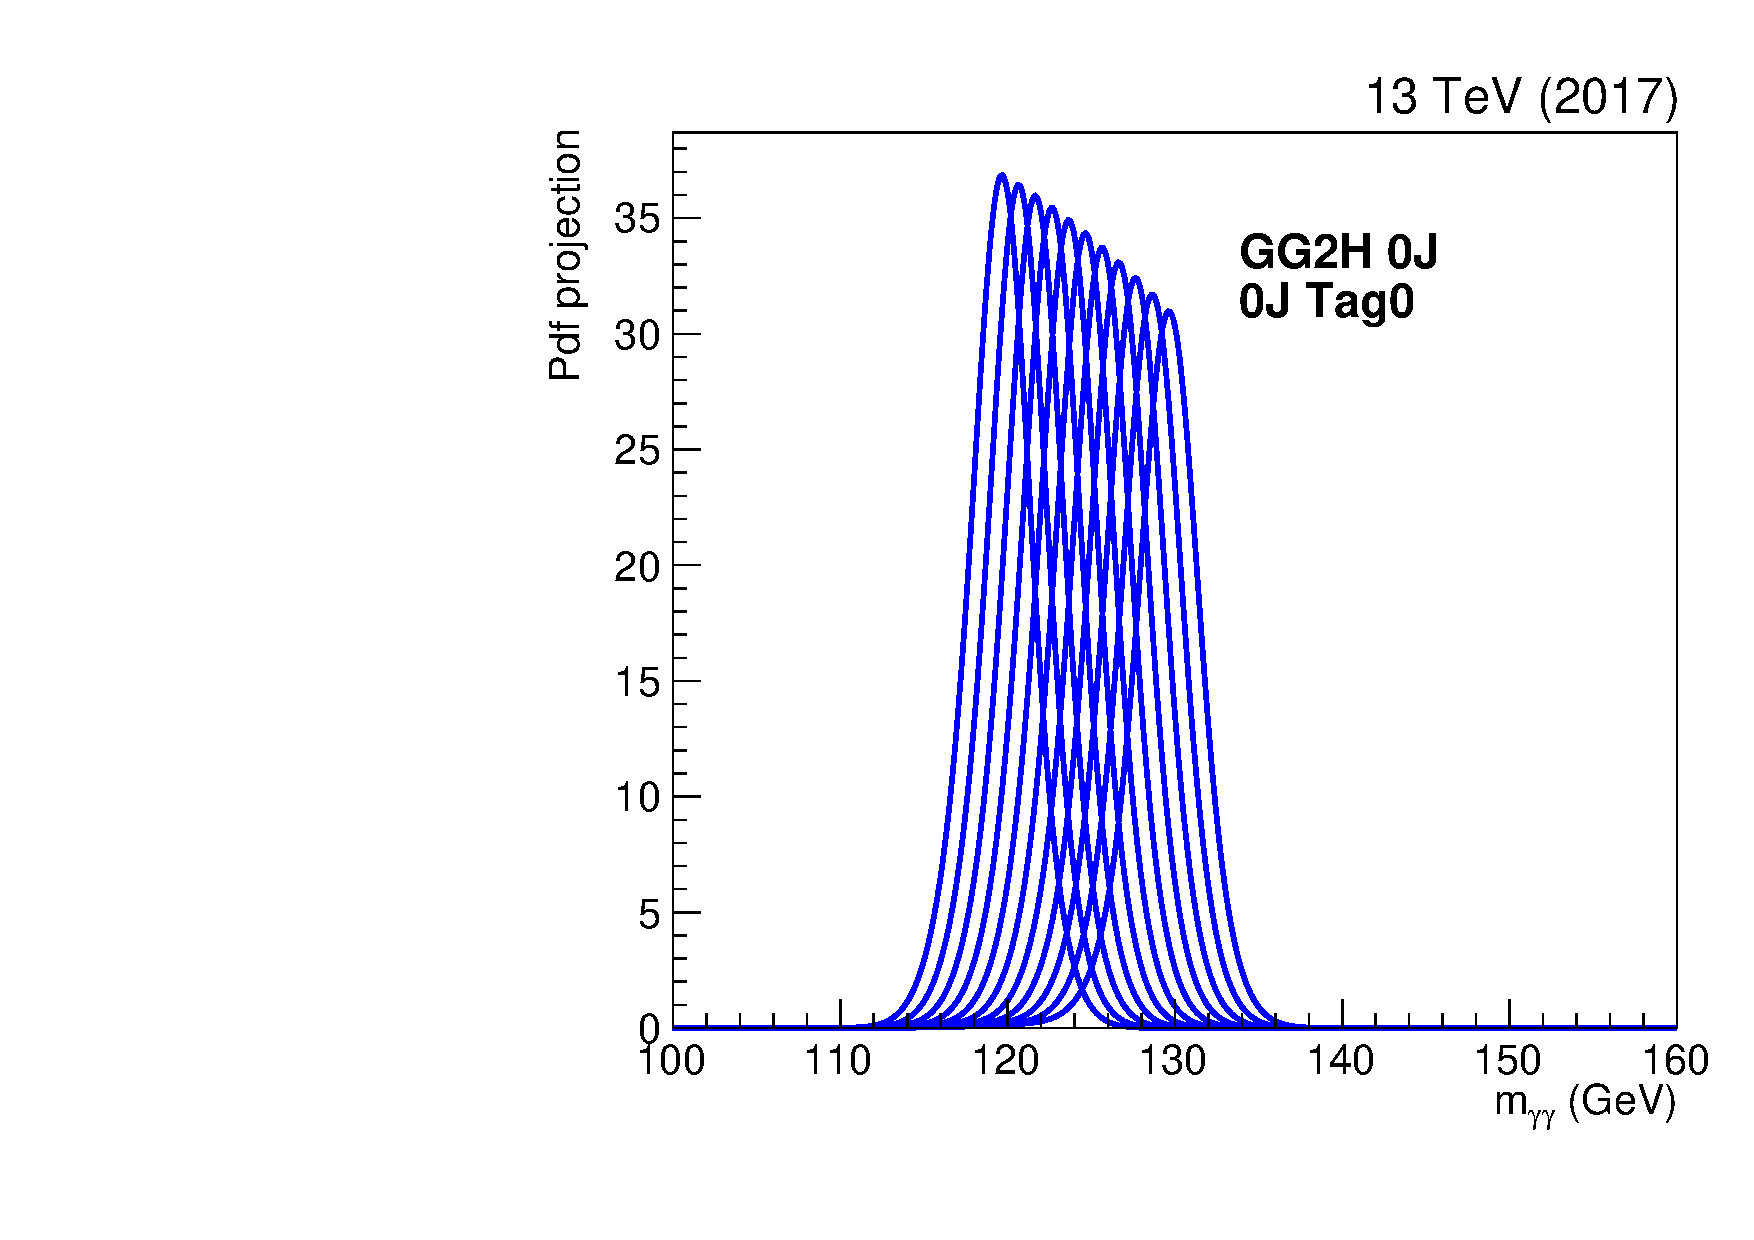
\includegraphics[width=0.49\textwidth]{Figures/SigBkg/GG2H_0J_RECO_0J_Tag0_interp_2017.pdf}
  \caption[Parametric signal model as a function of \mH.]
  {
    The evolution of the parametrised signal model shape as a function of \mH.
    The plots show the signal model for the ggH 0J bin in the 0J Tag 0 category.
    The left plot shows 2016 simulation, with 2017 simulation on the right.
  }
  \label{fig:sigbkg_interp}
\end{figure}

In some cases, there is an insufficient number of simulated events available 
to accurately model the shape for a given combination of stage 1 bin, 
analysis category and vertex scenario. %threshold on nEvents set at 200
The shape is then replaced by that of the stage 1 bin 
which has the highest expected yield in the category under consideration.
This replacement procedure is motivated by the fact that events subject to the same selection
tend to have similar values of the diphoton mass resolution.

After each model has been constructed, the shapes from the RV and WV scenarios are combined.
The fraction of events in which the correct vertex is chosen 
is also described by a linear function of \mH; 
once determined, this is used to assign the correct normalisations for the RV and WV models.
An example of the signal model for the ggH 0J bin in the 0J Tag 0 category, 
after the models for the RV and WV scenarios have been summed,
is shown in Figure~\ref{fig:sigbkg_proccat}.

\begin{figure}[hptb]
  \centering
  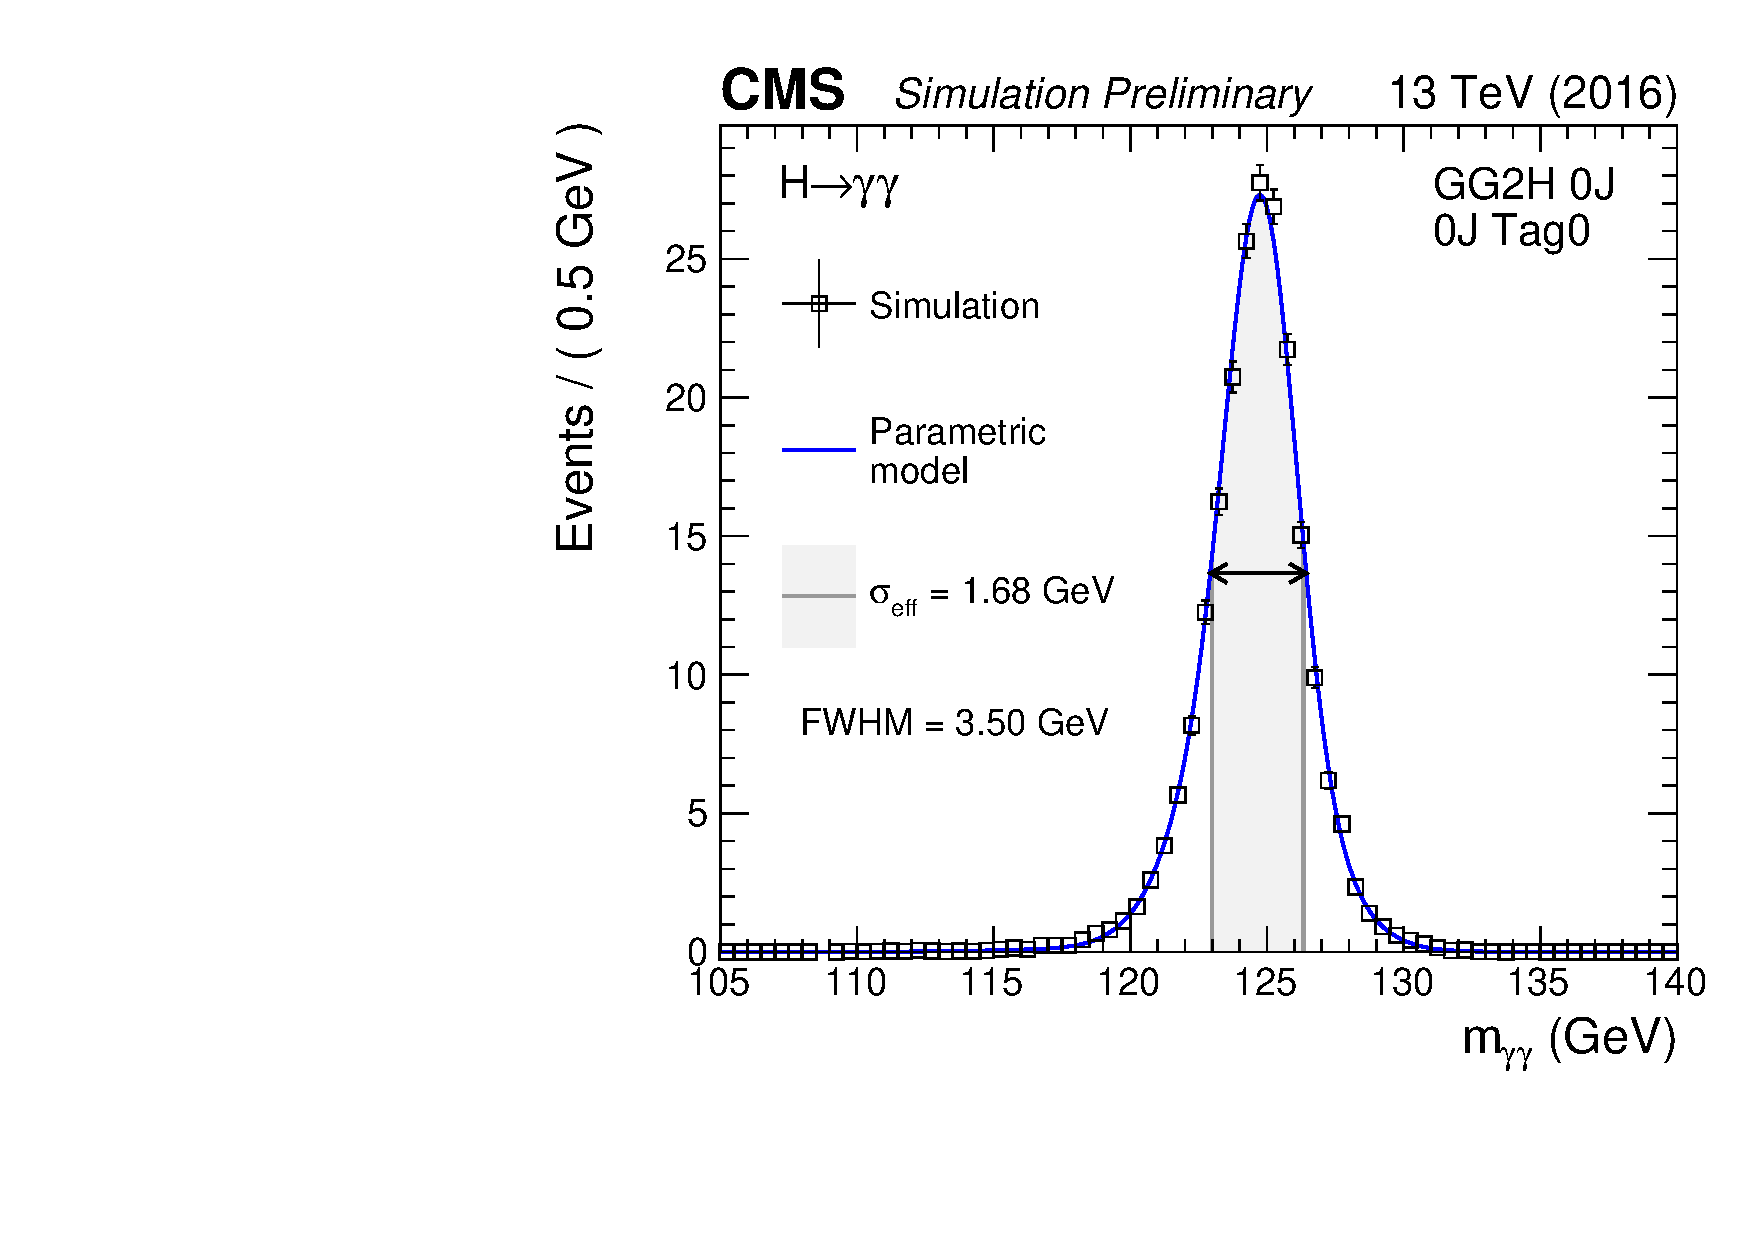
\includegraphics[width=0.49\textwidth]{Figures/SigBkg/GG2H_0J_RECO_0J_Tag0_2016.pdf}
  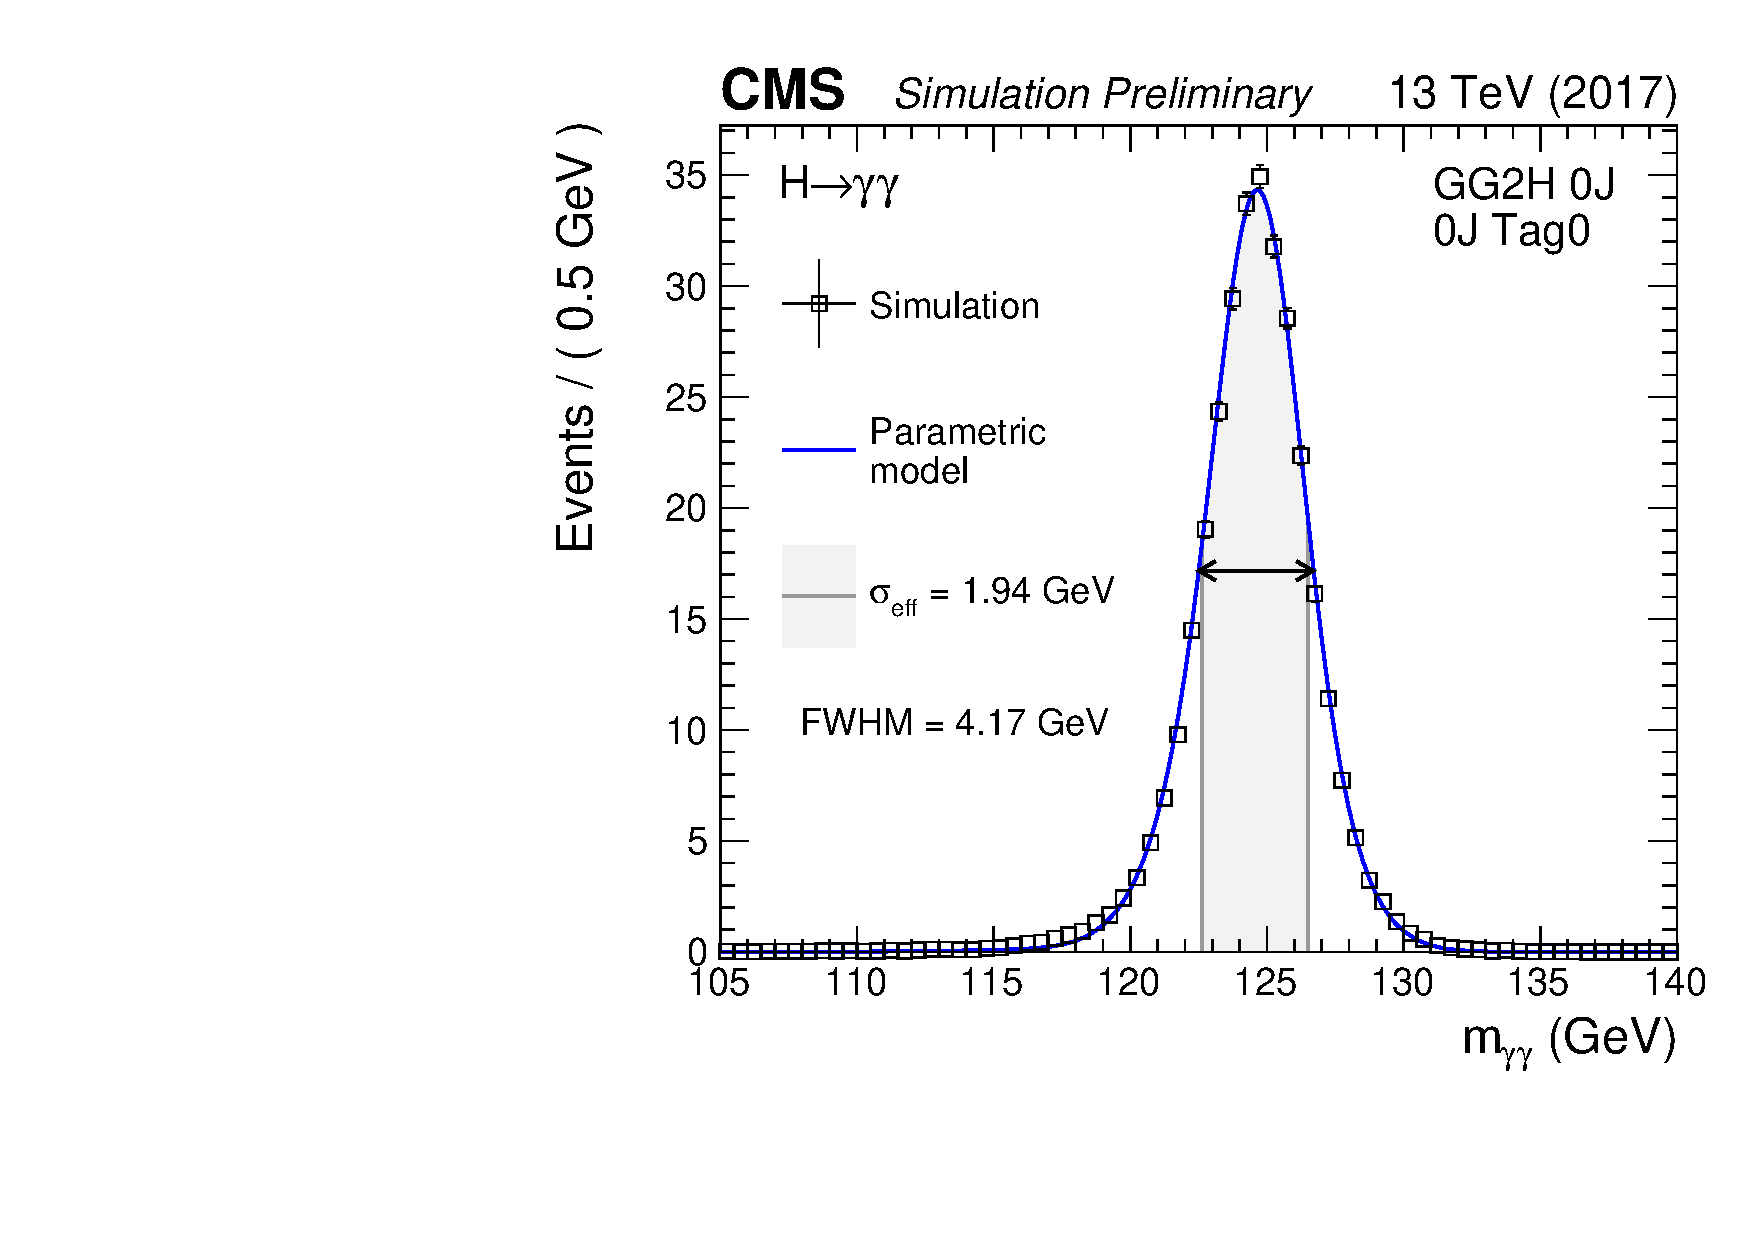
\includegraphics[width=0.49\textwidth]{Figures/SigBkg/GG2H_0J_RECO_0J_Tag0_2017.pdf}
  \caption[Signal model for the ggH 0J bin in the 0J Tag 0 category.]
  {
    The parametrised signal shape for the ggH 0J bin in the 0J Tag 0 category, 
    after the models for the RV and WV scenarios have been summed.
    The open squares represent weighted simulation events and the blue line the
    corresponding model. Also shown is the \seff value (half the width of the narrowest interval
    containing 68.3\% of the invariant mass distribution) and the full width at half of the maximum
    (FWHM). The left plot shows 2016 simulation, with 2017 simulation on the right.
  }
  \label{fig:sigbkg_proccat}
\end{figure}

For each category, 
the models corresponding to the contributions from each stage 1 bin are then summed.
To normalise the contribution from each stage 1 bin correctly, 
the total number of expected events for each stage 0 process is obtained 
using the cross sections and \Hgg branching ratio from Ref.~\cite{YR4}\footnote{The exception is ggH, 
for which the latest calculations at N3LO are used \cite{Anastasiou2015,Anastasiou2016}.},
and the measured integrated luminosity in data.
The fraction of each stage 1 bin is then taken from the simulated events for each stage 0 process.
Finally, the product of the detector efficiency and analysis acceptance 
is modelled as a linear function of \mH, 
determined by the ratio of the total number of expected events 
to the number of events entering each analysis category.
Together these allow the total signal model for each category to be computed.
An example of the signal model for the 0J Tag 0 category, 
after the models for all the stage 1 bins have been summed, 
is shown in Figure~\ref{fig:sigbkg_cat}.

\begin{figure}[hptb]
  \centering
  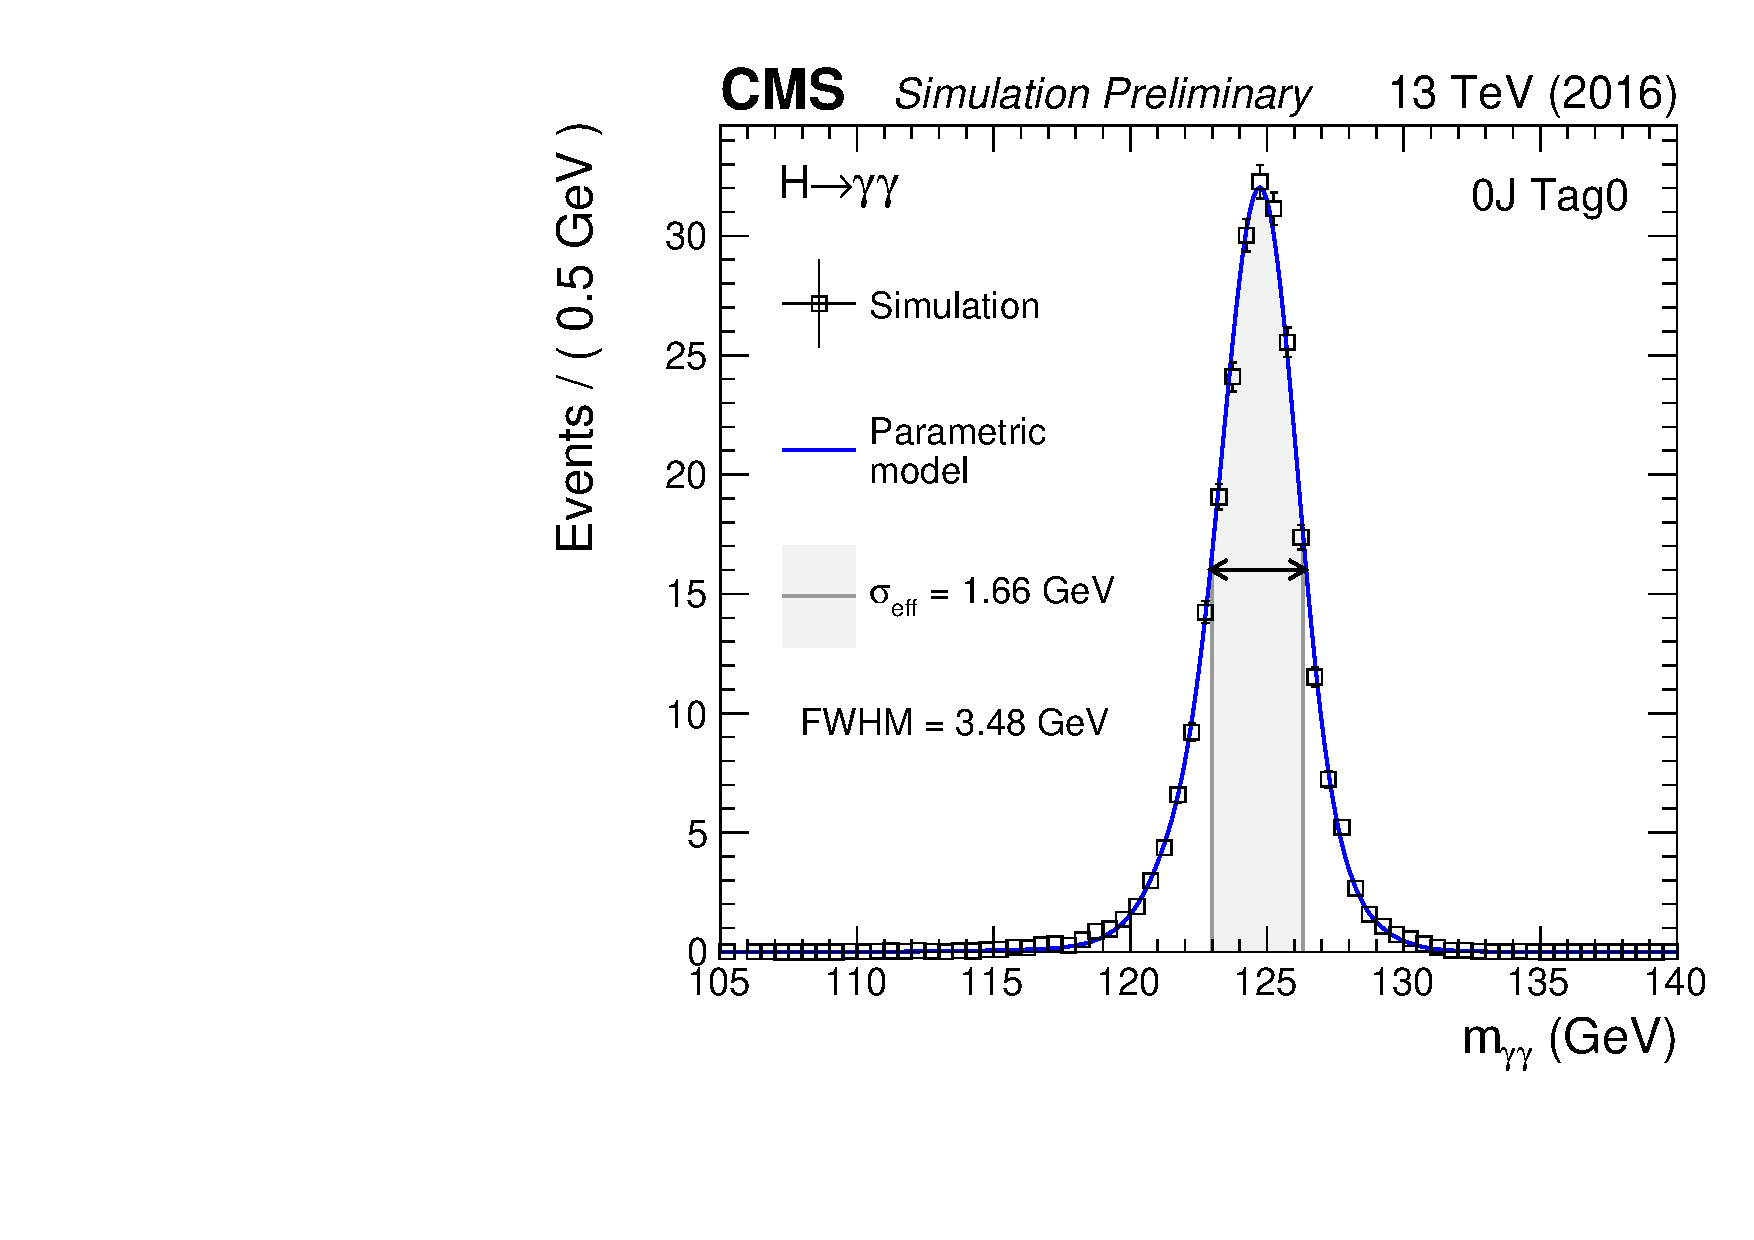
\includegraphics[width=0.49\textwidth]{Figures/SigBkg/RECO_0J_Tag0_2016.pdf}
  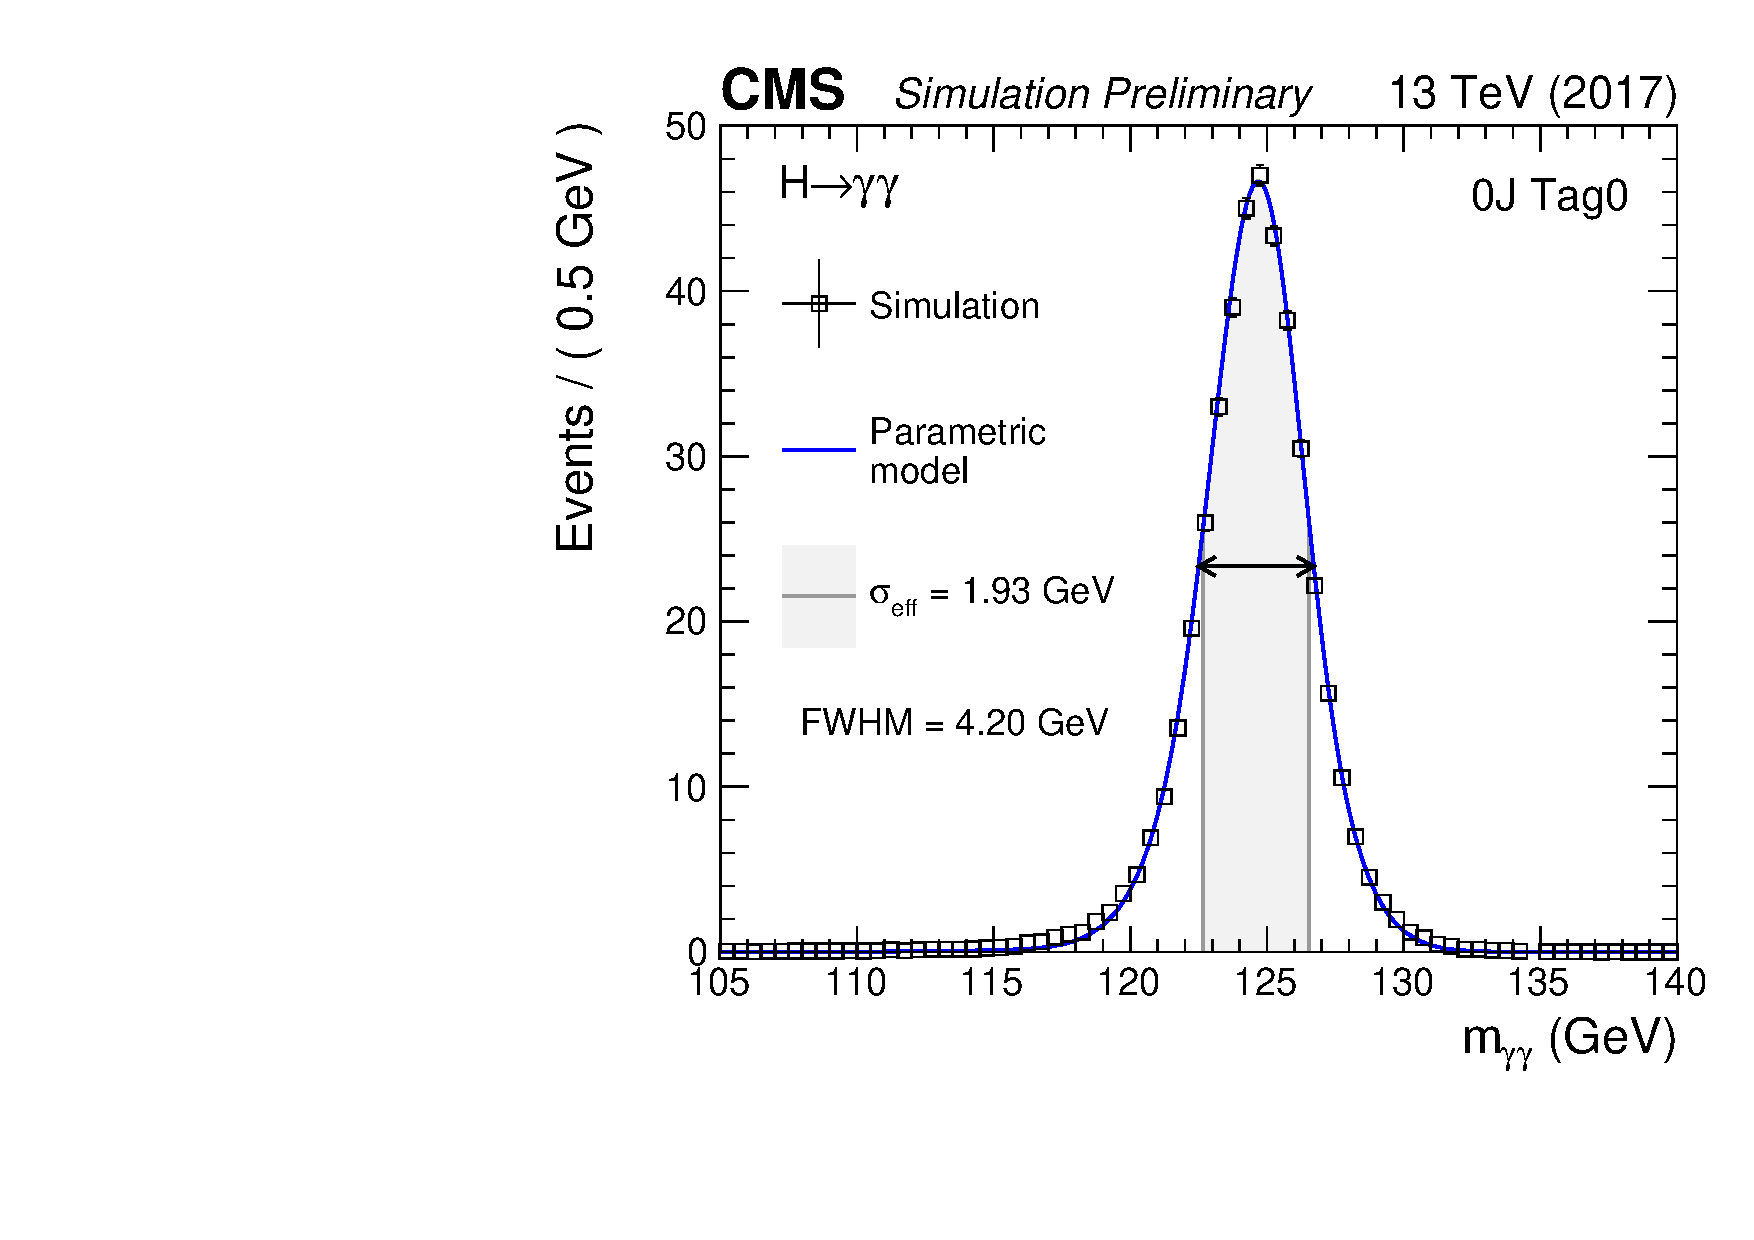
\includegraphics[width=0.49\textwidth]{Figures/SigBkg/RECO_0J_Tag0_2017.pdf}
  \caption[Signal model for the 0J Tag 0 category.]
  {
    The parametrised signal shape for the 0J Tag 0 category, 
    after the models for all the stage 1 bins have been summed.
    The open squares represent weighted simulation events and the blue line the
    corresponding model. Also shown is the \seff value (half the width of the narrowest interval
    containing 68.3\% of the invariant mass distribution) and the full width at half of the maximum
    (FWHM). The left plot shows 2016 simulation, with 2017 simulation on the right.
    Figures first shown in Ref.~\cite{HIG-18-029}.
  }
  \label{fig:sigbkg_cat}
\end{figure}

\section{Background modelling}

The background model represents the smoothly falling spectrum 
in the \mgg distribution that results from processes other than Higgs boson production.
The shape of this falling distribution is not known a priori;
therefore different functional forms must be considered when constructing the model.
Each choice of function results in a different number of estimated events 
under the signal peak produced by the Higgs boson, 
and hence affects the measured value of parameters representing the size of the signal contribution.
The uncertainty in the measurement associated with this choice must be accounted for 
in the final results.
In this analysis, the discrete profiling method is used, as first described in Ref.~\cite{Envelope}.
The model is constructed independently for each analysis category.

The discrete profiling method incorporates the uncertainty on the background 
into the measurement by treating the choice of function used to model the background distribution
as a discrete nuisance parameter.
Ordinarily, a nuisance parameter is a continuous variable which affects the measured value 
but is not in itself of any interest.
The choice of background function can be treated in the same way as any other nuisance parameter, 
with the only difference being that its value is discrete rather than continuous.
To construct the final 2NLL curve, 
the so-called ``envelope" of all the possible choices of background function is taken.
This procedure is illustrated in Figure~\ref{fig:sigbkg_envelope}, 
which shows how the 2NLL curve for the fully profiled fit can be approximated 
by taking the envelope of the curves generated with a nuisance parameter fixed to different values.
The discrete profiling method accounts for the uncertainty in the background function analogously;
a different curve is generated by each choice of background function, 
and the final curve represents the envelope of each of these individual curves.
This envelope is necessarily wider than any of the curves corresponding to an individual function, 
and therefore returns a greater uncertainty, 
reflecting the imperfect knowledge of the shape of the background distribution.

\begin{figure}[hptb]
 \centering
 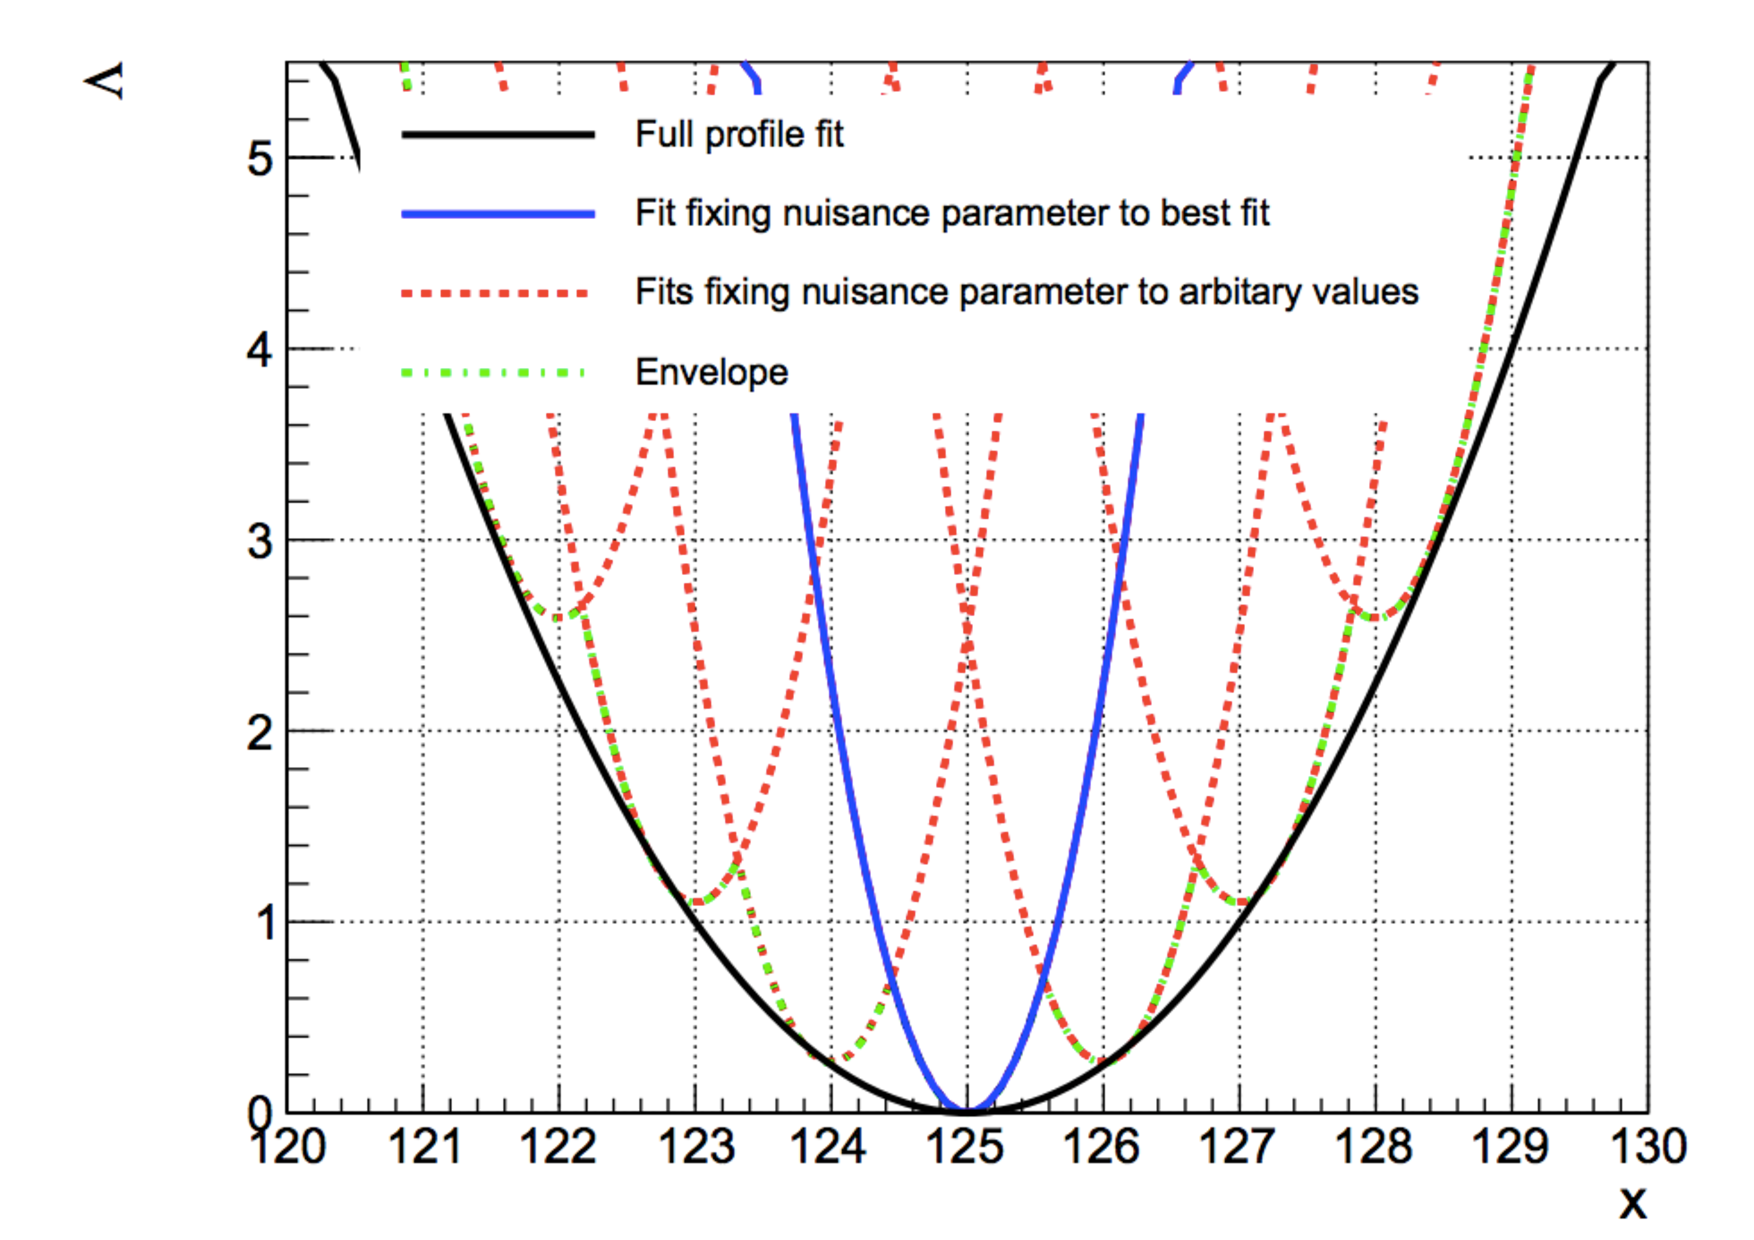
\includegraphics[width=\textwidth]{Figures/SigBkg/EnvelopeIllustration.pdf}
 \caption[Illustration of the discrete profiling method.]
 {
   An illustration of the discrete profiling, or envelope, method.
   The envelope of all the curves corresponding to fixed values of a given nuisance parameter
   approximates the full curve obtained when the nuisance parameter is profiled.
   Figure taken from Ref.~\cite{Envelope}.
 }
 \label{fig:sigbkg_envelope}
\end{figure}

In principle, all functions which provide a sufficiently good fit to the observed \mgg distribution
in data could be included in the discrete profiling method.
To apply the method in practice, 
four different families of functions representing smoothly falling distributions are considered.
These groups, 
for an $N$-parameter function with parameters $p_0, p_1, ..., p_N$ to be determined, are: 
\begin{itemize}
\item Sum of exponential functions, where
\begin{equation*}
f_N(x) = \sum_{i=0}^{N} p_{2i}\exp{\left(p_{2i+1}x\right)}
\end{equation*}
\item Sum of power law functions, where
\begin{equation*}
f_N(x) = \sum_{i=0}^{N} p_{2i}\,x^{-p_{2i+1}}
\end{equation*}
\item Bernstein polynomials, where
\begin{equation*}
f_N(x) = \sum_{i=0}^{N} p_{i}\binom{N}{i}x^{i}\left(1-x\right)^{N-i}
\end{equation*}
\item Laurent series, where
\begin{equation*}
f_N(x) = \sum_{i=0}^{N} p_{i}\,x^{-4 + L(i)},
\end{equation*}
with
\begin{equation*}
L(i) = \sum_{j=0}^{i}(-1)^j j .
\end{equation*}
\end{itemize}

Only a subset of functions from each family are considered;
this is necessary to maintain a reasonable computational efficiency for the method.
For each family of functions, multiple orders can be included in the final set of candidate functions.
A likelihood fit is performed for each order, 
and then the procedure to decide which orders to include works as follows.
A penalty equal to the number of parameters in the function is added to the value of the 2NLL;
this prevents functions of arbitrarily high order being chosen.
First, the order is increased until a minimum goodness-of-fit threshold is reached;
there is no need to include functions which do not fit the data well. %threshold is 0.01 from chisq
For each subsequent order, an F-test \cite{Fisher} is performed to gauge the size of the improvement in the fit
quality which the increase in function complexity brings.
This test computes a $p$-value by assuming the difference in 2NLL values 
is distributed as a $\chi^2$, with degrees of freedom equal to 
the difference in number of parameters between the two orders.
If the $p$-value is below a certain threshold, %threshold value 0.05
the higher order function is deemed to constitute a worthwhile improvement, 
is added to the set of functions considered, and the process continues.
Otherwise, the higher order function is not included and the procedure is complete.
The different functions chosen for the 1J high Tag 0 category 
are shown in Figure~\ref{fig:sigbkg_functions};
it can be seen that different choices of function lead to a different number of events 
when integrating under the signal peak.
In this case, the range in the integrated number of events around the Higgs boson mass
amongst the candidate functions shown is of the order ten.

\begin{figure}[hptb]
  \centering
  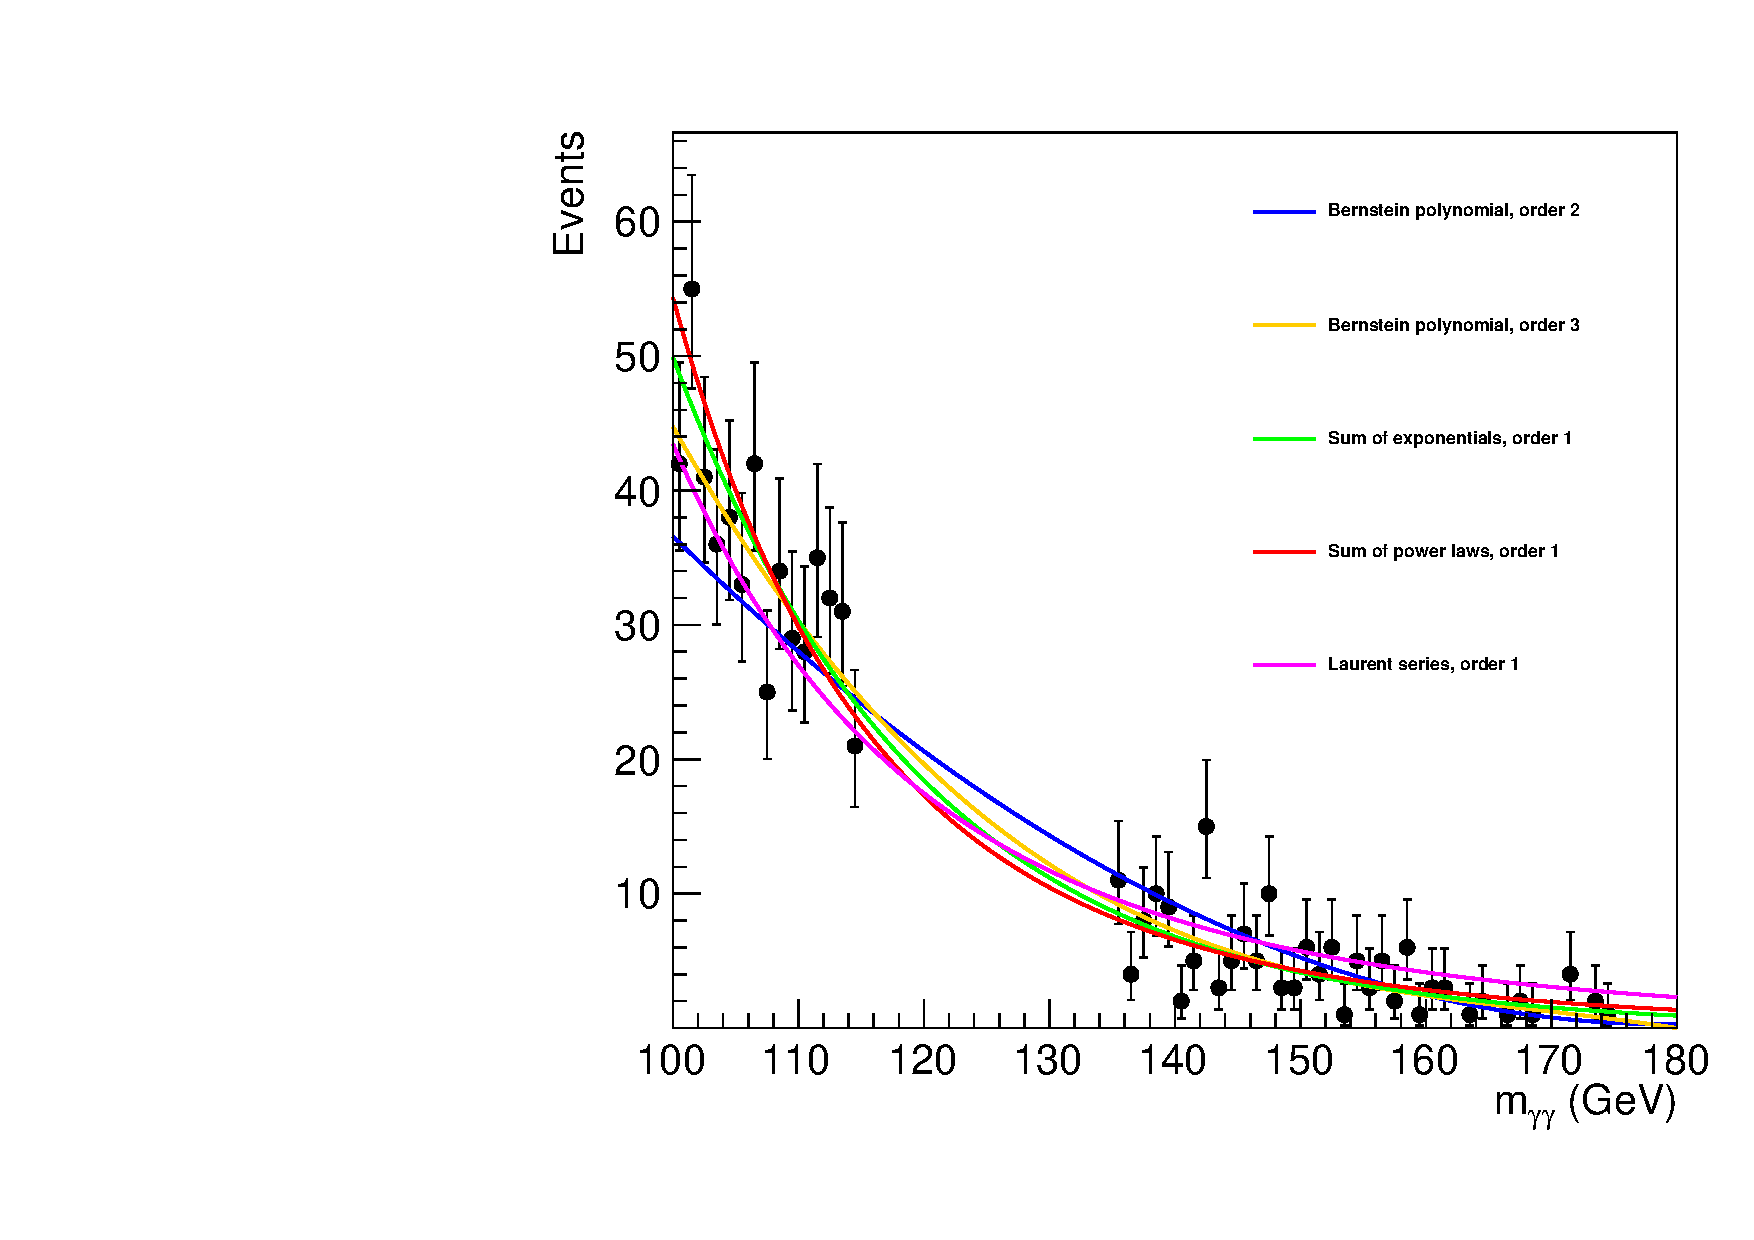
\includegraphics[width=0.49\textwidth]{Figures/SigBkg/allPdfs_RECO_1J_PTH_120_200_Tag0_2016.pdf}
  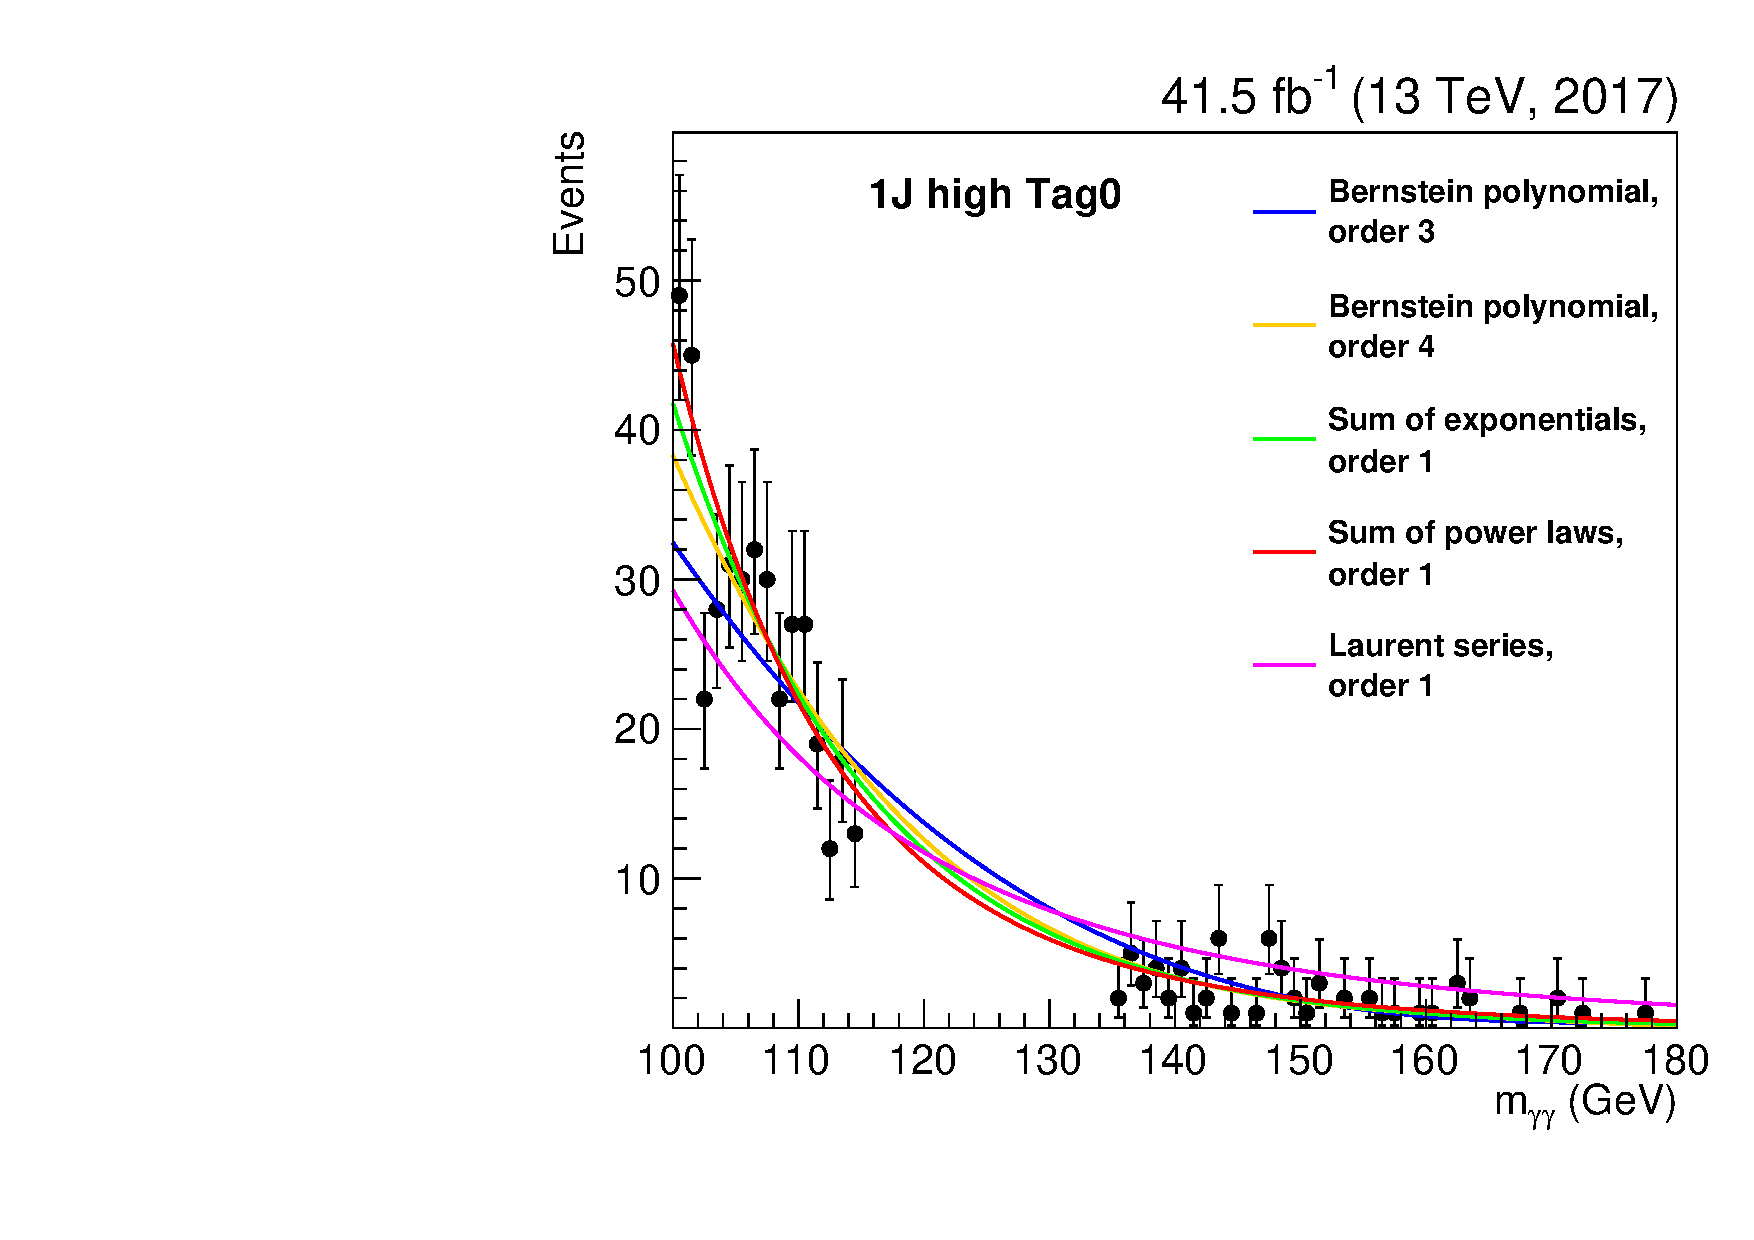
\includegraphics[width=0.49\textwidth]{Figures/SigBkg/allPdfs_RECO_1J_PTH_120_200_Tag0_2017.pdf}
  \caption[Candidate background functions considered for the 1J high Tag 0 category.]
  {
    The functions chosen for consideration in the final fit for the 1J high Tag 0 category, 
    with the data (black points) blinded, 
    meaning the points with $115 < \mgg < \SI{135}{GeV}$ are not shown.
    The left plot shows 2016 data, with 2017 data on the right.
  }
  \label{fig:sigbkg_functions}
\end{figure}

In the final fit, the background function is chosen from the set of candidates as described above.
All parameters of each function are free to vary and determined in the fit.
As for the F-test above, 
a regularisation term is added to the 2NLL for each parameter in the chosen function.
This serves to penalise unnecessary complexity.
Further details of the discrete profiling method, 
including studies of the bias and coverage,
are contained within Ref.~\cite{Envelope}.

\section{Systematic uncertainties}

In this analysis, the systematic uncertainty associated with the data-driven background estimation 
is handled using the discrete profiling method, as described above.
There are many systematic uncertainties which affect the signal model; 
these are handled in one of two ways.
Uncertainties which modify the shape of the \mgg distribution are incorporated into the signal model
as nuisance parameters, where the mean and width of each Gaussian function can be affected.
These uncertainties are typically experimental uncertainties 
relating to the energy of the individual photons. 
Conversely if the shape of the \mgg distribution is unaffected, 
the uncertainty is treated as a log-normal variation in the event yield.
These uncertainties include theory sources
and experimental uncertainties such as those affecting the BDTs used for categorising events.
The magnitude of each uncertainty's impact is determined individually 
for each stage 1 bin in each analysis category.
%For log-normal nuisances this impact can be either symmetric or asymmetric,
%in the latter case depending on whether the uncertainty is varied in the up or down direction.

\subsection{Theoretical uncertainties}

The sources of theoretical uncertainties considered in this analysis are as follows:
\begin{itemize}
\item \textit{QCD scale uncertainty}: 
  the uncertainty arising from variations of the renormalisation and factorisation scales
  used when computing the expected SM cross section and event kinematics.
  These account for the missing higher order terms in perturbative calculations.
  The recommendations provided in Ref.~\cite{YR4} are followed.
  This involves estimating the uncertainty using three sources: 
  varying the renormalisation by a factor of two, varying the factorisation scale by a factor of two, 
  and varying both in the same direction simultaneously.
  Depending on the production process, the size of the uncertainty varies from around 0.5\% 
  to 9\%.
\item \textit{Uncertainty on the SM ggH production}: 
  for ggH production, 
  additional sources are included which account for the uncertainty in the modelling 
  of the \ptH distributions, the number of jets in the event, 
  and the ggH contamination in the VBF categories.
  Two sources reflect the migration uncertainty around the \ptH bin boundaries,
  at 60 and 120 GeV respectively; 
  their magnitude depends on the number of jets and the \ptH in the event.
  An additional source covers the uncertainty on \ptH 
  arising from the treatment of the top quark mass in the ggH loop.
  Two further sources account for the migration between the zero, one and two or more jet bins.
  The uncertainty on the ggH production of events with a VBF-like dijet system 
  is covered by two sources 
  corresponding to the prediction in the two-jet-like and three-jet-like bins.
  The total magnitude of these uncertainties vary from around 5\% to 30\%, 
  with events that have one or more jets and high values of \ptH 
  typically having the greatest associated uncertainty.
\item \textit{PDF (parton density functions) uncertainties}:
  these account for the uncertainty due to imperfect knowledge of the composition of the proton, 
  which affects which partons are most likely to initiate high energy events.
  The overall normalisation uncertainties are computed
  following the PDF4LHC
  prescription~\cite{PDF4LHC,YR3},
  while the bin-to-bin migrations are calculated from the
  NNPDF3.0~\cite{NNPDF3} PDF set
  using the {\sc MC2hessian} procedure~\cite{MC2Hessian}.
  The overall normalisation uncertainties are between 1-5\%, 
  with the migrations significantly smaller, usually less than 1\%.
\item \textit{Uncertainty in the strong force coupling constant}: 
  the uncertainty in the value of the strong force coupling constant $\alpha_{s}$ 
  is included in the treatment of the PDF uncertainties, following the PDF4LHC prescription.
\item \textit{Uncertainty in the \Hgg branching fraction}: 
  the probability of the Higgs boson decaying to two photons is required to calculate
  the SM expected cross section, but this branching fraction is not known exactly.
  The uncertainty is currently estimated to be 2\%~\cite{YR4}.
\item \textit{Underlying event and parton shower uncertainties}: 
  these uncertainties are obtained using dedicated simulated samples 
  where the choice and specific tune of the event generator have been modified. 
  The impact of the uncertainty ranges from 1-16\% depending on the process and category.
\end{itemize}

The QCD scale and PDF uncertainties impact the theoretical modelling in two ways.
Both the overall cross section prediction for a given STXS bin, 
and the distributions of kinematic variables used in the event selection and categorisation,
can be affected.
The effects on the overall process cross section predictions are omitted 
when measurements of simplified template cross sections are performed,
and are instead considered as uncertainties on the SM prediction.
However the uncertainties on the event kinematics, 
which affect the efficiency and acceptance of the analysis, 
are still taken into account.
All uncertainties are included when measurements of signal strength modifiers are performed.
Other uncertainties which only affect the overall SM predicted yields, 
such as the \Hgg branching fraction, 
are also omitted from measurements of simplified template cross sections.

\subsection{Experimental uncertainties}

The uncertainties which affect the shape of the signal \mgg distribution are:
\begin{itemize}
\item \textit{Photon energy scale and resolution}: 
  the uncertainties associated with the corrections applied to the photon energy scale in data
  and the resolution in simulation are evaluated using \Zee events.
  The estimate is computed by varying the regression training scheme, the \RNINE variable, 
  and the electron selection criteria.
\item \textit{Non-linearity of the photon energy scale}: 
  a further source of uncertainty covers possible remaining differences in the linearity 
  of the photon energy scale between data and simulation.
  The uncertainty is estimated using boosted \Zee events.
\item \textit{Modelling of electromagnetic showers}: 
  this uncertainty accounts for the imperfect knowledge of electromagnetic showering processes.
  The size of the effect is estimated by changing the model used to generate 
  the bremsstrahlung energy spectrum, which can modify the photon and electron energy scales.
\item \textit{Shower shape corrections}: 
  an uncertainty on the shower shape corrections accounts for the imperfect modelling 
  of shower shapes in simulation.
  The impact is estimated by comparing the energy scale before and after 
  the corrections to shower shape variables 
  (which improve the agreement between data and simulation) are applied.
\item \textit{Light collection non-uniformity}: 
  an uncertainty is associated with the modelling of the light collection 
  as a function of emission depth within a given ECAL crystal.
  It is estimated by comparing simulation with analytical estimates of longitudinal shower profiles.
  %TODO check if the above is even close to true
\item \textit{Modelling of material in front of the ECAL}: 
  the amount of material through which objects pass before reaching the ECAL 
  affects the behaviour of the electromagnetic showers, 
  and may not be perfectly modelled in simulation.
  Dedicated samples with variations in the amount of upstream material are used to 
  estimate the impact on the photon energy scale.
\item \textit{Vertex fraction}: 
  the largest contribution to the right and wrong vertex fraction 
  uncertainty comes from the modelling of the underlying event, in addition to 
  the uncertainty on the ratio of data and simulation obtained using
  \Zmumu events. It is handled as an additional
  nuisance parameter built into the signal model which allows the fraction
  of events in the right vertex/wrong vertex scenario to change.
\end{itemize}

The uncertainties which only modify the event yield include:
\begin{itemize}
\item \textit{Integrated luminosity}: 
  estimated to be 2.5\% and 2.3\% for the 2016 and 2017 datasets respectively \cite{Lumi2016,Lumi2017}.
\item \textit{Photon identification BDT score}: 
  the uncertainty arising from the photon identification BDT score 
  is estimated by requiring the systematic variation 
  to cover the observed discrepancies between data and simulation. 
  This is described further in Chapter~\ref{chap:objects}.
  The uncertainty on the signal yields is
  estimated by propagating this uncertainty through the full category selection procedure.
  The impact in the most sensitive analysis categories is around 5\%.
\item \textit{Jet energy scale and smearing corrections}: 
  The energy scale of jets is measured using the \pt balance of jets with Z bosons and photons in
  \Zee, \Zmumu and $\gamma$+jets events, as well as the \pt balance between jets 
  in dijet and multijet events \cite{JetsInRun2}. The uncertainty in the jet energy scale
  is a few per-cent and depends on \pt and $\eta$. The impact of jet energy scale uncertainties on 
  event yields is evaluated by varying the jet energy corrections within their uncertainties and 
  propagating the effect to the final result.
  The resulting uncertainty in the final analysis categories can be as high as 21\% 
  for the scale, but is less than around 4\% for the resolution.
\item \textit{Per-photon energy resolution estimate}: 
  the uncertainty on the per-photon resolution is
  parametrised as a rescaling of the resolution by
  $\pm 5\%$ about its nominal value. 
  This is designed to cover all differences between data and simulation 
  in the distribution, which is an output of the energy regression.
\item \textit{Trigger efficiency}: 
  the efficiency of the trigger selection is measured with 
  $\Zee$ events using the tag-and-probe technique.
  The size of its uncertainty is less than 1\%.
\item \textit{Photon preselection}: 
  the uncertainty on the preselection efficiency
  is computed as the ratio between the efficiency measured in data and in simulation.
  Its magnitude is less than 1\%.
\item \textit{Missing transverse energy}: 
  this uncertainty is computed by shifting the
  reconstructed $\pt$ of the particle candidates entering the
  missing transverse energy computation, 
  within the momentum scale and resolution uncertainties appropriate 
  to each type of reconstructed object,
  as described in Ref.~\cite{JetsInRun2}.
  In this analysis, the size of the uncertainty is very small.
\item \textit{Pileup jet identification}: 
  the uncertainty on the pileup jet classification output score is estimated by
  comparing the score of jets in events with a Z boson and one balanced jet
  in data and simulation. 
  The magnitude is of the order 1\%.
\item \textit{Lepton isolation and identification}: 
  this uncertainty affecting electrons and muons
  is computed by varying the ratio of the efficiencies and
  using the tag and probe technique in \Zee events. 
  The resulting impact on the categories selecting leptons is up to around 3\%.
\item \textit{Efficiency of b-tagging}: 
  uncertainties on the b-tagging efficiency are evaluated 
  by comparing data and simulated distributions for the b-tag
  discriminator.
  The uncertainties include the statistical component on the
  estimate of the fraction of heavy and
  light flavour jets in data and simulation.
  Its magnitude is around 1\%.
\end{itemize}

\subsection{Correlation of uncertainties}

Since the analysis inputs and category definitions are constructed independently 
for the 2016 and 2017 datasets, %ie add in quadrature or linearly, assuming no constraint
the uncertainties affecting each year can either be chosen to be correlated or uncorrelated.
If an uncertainty is deemed to be correlated, 
then there is only one nuisance parameter in the final fit 
whose value will affect both the 2016 and 2017 categories.
Otherwise, if the uncertainties are uncorrelated, there is a separate nuisance parameter for each year 
and the impact on the categories from each year is independent.

In this analysis, 
all the sources of theory systematic uncertainties are taken to be correlated between years.
In most cases this is clearly the correct treatment, %only e.g. UEPS which might not be
since the underlying theoretical predictions are the same for each year 
and independent of the data-taking conditions.
For the experimental uncertainties,
most uncertainties are left uncorrelated.
This is motivated by the fact that both the data-taking conditions 
and the reconstruction vary between the two years.
An exception is the uncertainty on the photon identification BDT output, 
which is kept correlated because the uncertainty prescription is identical for both years.
The final results were also computed with all the experimental uncertainties taken to be correlated, 
and it was confirmed that the difference between the two correlation scenarios is minimal.
This is in accordance with expectation, since the predominant source of uncertainty 
in all the stage 1 measurements is statistical in origin.

\section{Summary}

The inputs to the final fits of this analysis are the simulated signal model 
and the data-driven background model.
The uncertainty on the background model is accounted for using the discrete profiling method, 
where the choice of background function is treated as a nuisance parameter.
The signal model is parametric in \mH, 
with the contribution from each stage 1 bin in each analysis category modelled separately.
There are numerous uncertainties included in the signal model, 
which either affect the shape of the signal mass distribution 
or the event yield.
An illustration of the impact of the systematic uncertainties 
on different signal strength measurements, 
from the previous CMS \Hgg analysis documented in Ref.~\cite{HIG-16-040}, 
is shown in Figure~\ref{fig:sigbkg_systematics}.
The systematic uncertainties with the greatest impact on the inclusive Higgs boson signal strength
are the photon identification uncertainty and theoretical sources relating to ggH production.
In contrast, the leading systematic uncertainties affecting VBF signal strength measurement 
are those on the jet energy scale and resolution corrections.
The same sources of systematic uncertainties are included in this analysis.
The precision of the measurements of stage 1 simplified template cross sections presented here
is limited by statistical uncertainties.
However this will change as more data are collected, 
and once the full dataset from Run 2 is analysed 
the systematic uncertainties will become more important.

\begin{figure}[hptb]
  \centering
  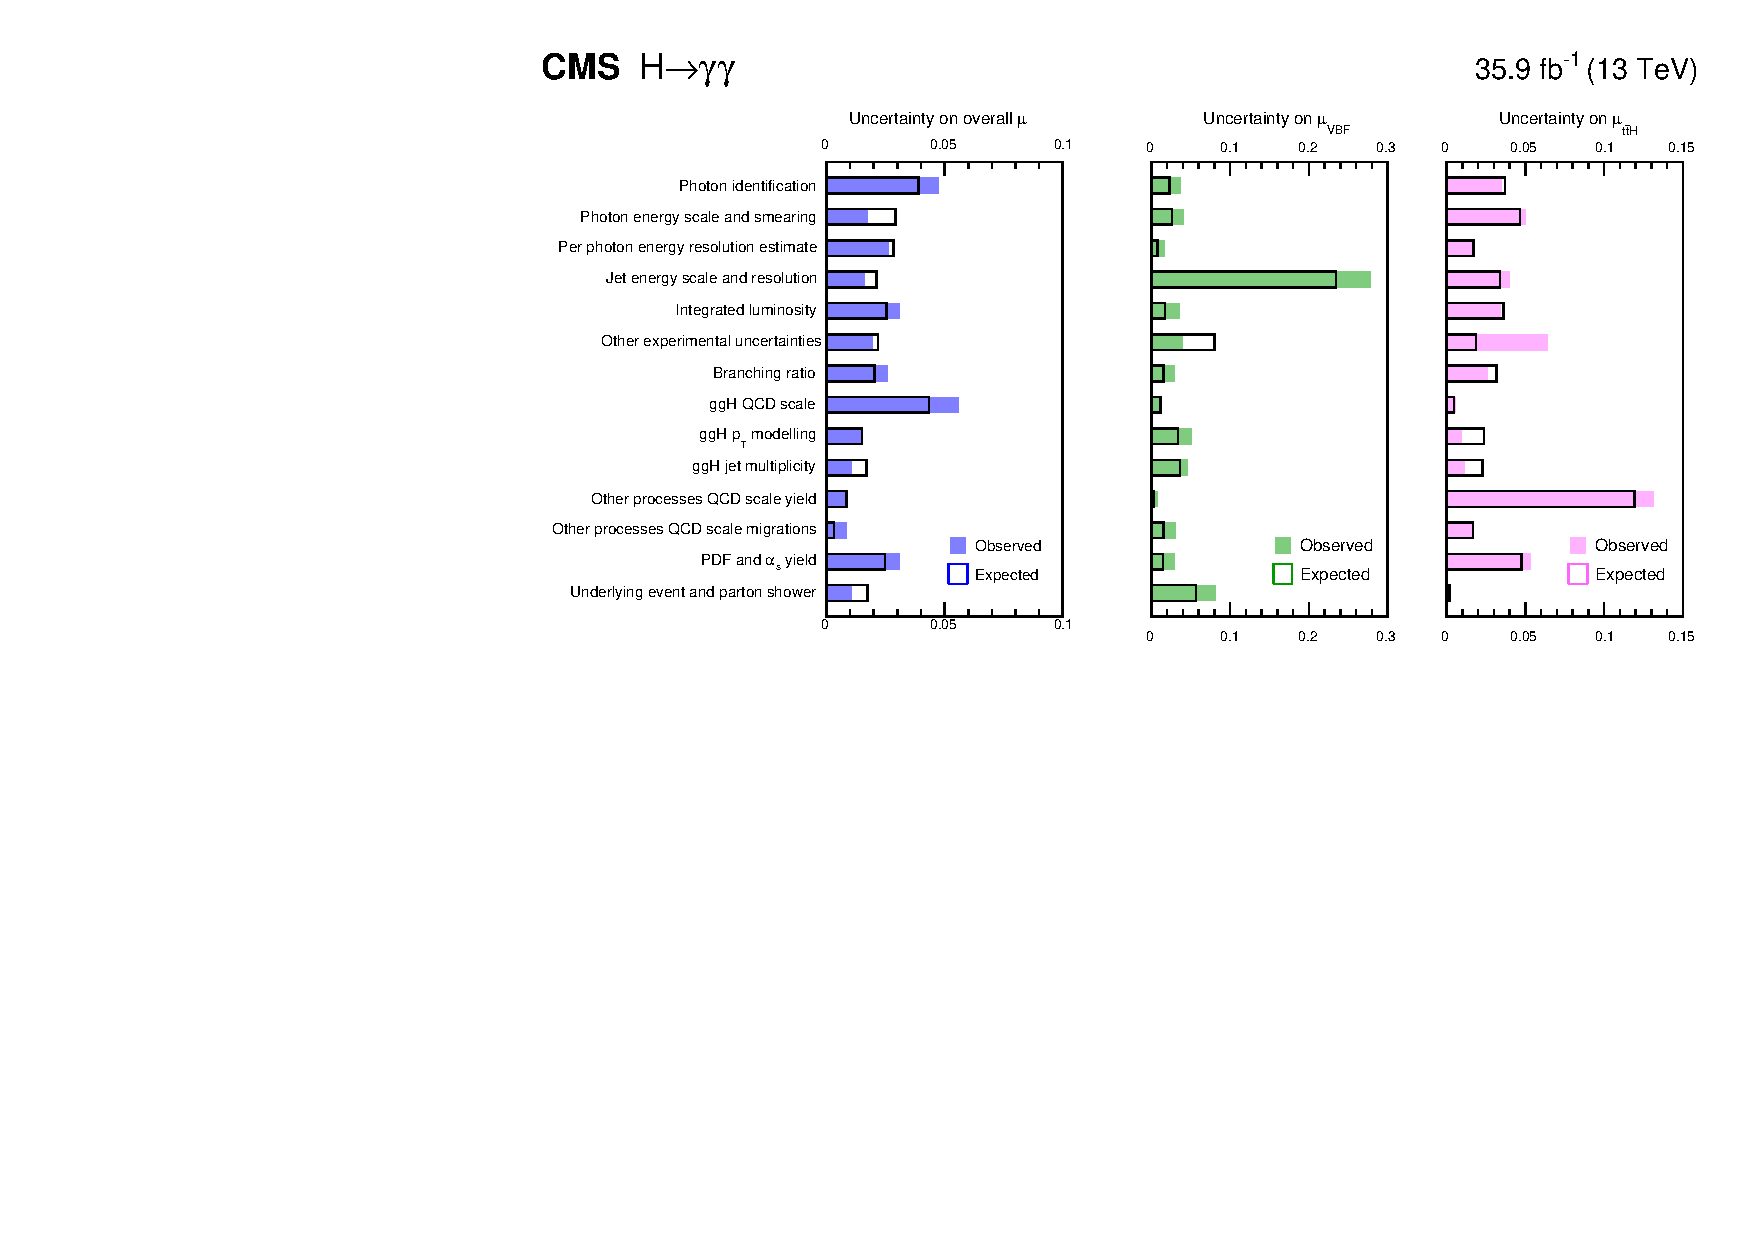
\includegraphics[width=\textwidth]{Figures/SigBkg/SystematicsTable.pdf}
  \caption[The impact of systematic uncertainties on signal strength measurements from Ref.~\cite{HIG-16-040}.]
  {
    The impact of the different systematic uncertainties on the inclusive, VBF, and ttH 
    signal strength modifiers in the previous CMS \Hgg analysis \cite{HIG-16-040}.
    The observed (expected) results are shown by the solid (empty) bars.
    This figure was first shown in Ref.~\cite{HIG-16-040}, 
    and is based on the results described therein.
  }
  \label{fig:sigbkg_systematics}
\end{figure}
